\chapter{Comparison of Multimodal Data Fusion Models for Predicting Survival Classification in Motor Neuron Disease}
\label{fusilli_on_mnd}

\section{Introduction}
Only one deep learning model has been used to predict survival in MND through clinical data and neuroimaging data~\cite{vanderburghDeepLearningPredictions2017}.
This lack of research in multimodal data fusion in MND makes it difficult to conclude whether multimodal data is useful in predicting survival in MND .
Additionally, we have shown that many different multimodal data fusion methods have been developed for other research applications.
In Chapter~\ref{fusilli_development}, we developed a package called Fusilli to compare the performance of multimodal data fusion methods, approximately half of which are designed to combine two tabular modalities.

In this chapter, we will use Fusilli to compare the performance of different tabular-tabular multimodal data fusion methods on predicting survival in MND patients using clinical and imaging extracted features data.
The aims of this work are to, firstly, assess the effect of different data fusion model architectures on prognostic performance, and secondly, to assess the value of baseline clinical and neuroimaging data in MND prognosis prediction.

\section{Data}

The data used in this analysis is from two studies: University College London Queen's Square Institute of Neurology's ALS Biomarkers Study~\cite{UKMNDCSG} and Ospedale San Raffaele's MND cohort.
Both of these datasets contain clinical data from the diagnostic visit and brain MRI data.

For patients to be included in the analysis, they must have a diagnosis of MND and have an outcome of interest (death or tracheostomy).
In the ALS Biomarkers Study, the outcome of interest is death, whereas in the Ospedale San Raffaele's MND cohort, the outcome of interest is death or tracheostomy.
Unfortunately, the Ospedale San Raffaele's MND cohort does not specify the date of death, so we have assumed that the date of death is the date of tracheostomy.

Patients in this analysis must have non-missing data for age at diagnosis, sex, date of diagnosis, date of death, date of symptom onset, site of onset, and baseline ALSFRS-R .
Additionally, patients must have a T1-weighted or T2-weighted MRI within 12 months before or after their date of diagnosis.

The final dataset contains 110 MND patients.
The patients in the cohort were split into two groups based on the median survival time: short survival group (less than 24 months) and long survival group (more than 24 months).

\subsection{Clinical Data}

The clinical variables chosen to be included in the analysis are based on the variables used in the ENCALS model~\cite{westenengPrognosisPatientsAmyotrophic2018} described in Chapter~\ref{literature_review}.
El Escorial criteria and FVC were not included in the analysis as they were not available in the Ospedale San Raffaele's MND cohort.
Features with missing data after the inclusion criteria were applied were features of FTD and presence of C9orf72 mutation.
Where these features were missing, they were assumed to be negative.
Moreover, where the MND type was missing, it was assumed to be ALS, as it is the most common.


\begin{table}
    \centering
    \caption{Differences in clinical demographics between the long and short survival groups. PRB is progression rate to baseline, calculated as the rate of decline of ALSFRS-R between symptom onset and diagnosis.\\
    *Chi-square test, \textdagger Fisher's exact test, $\ddagger$ Two-sample t-test.}
    \label{tab:clinical_demographics}
    \begin{tabular}{|p{4.3cm}|llll|}
    \hline
                                                        & \textbf{Overall}     & \textbf{Short}        & \textbf{Long}         & \textbf{P-Value}   \\
    \hline
     n                                                  & 110         & 55         & 55          &           \\ \hline
    \textbf{Categorical, n (\%)}                                &             &            &             &           \\ \hline
     Sex (Male)                                     & 52 (47.3)   & 27 (49.1)  & 25 (45.5)   & 0.849*     \\ \hline
     Bulbar Onset                          & 31 (28.2)   & 20 (36.4)  & 11 (20.0)  & 0.090*     \\\hline
     FTD                      & 32 (29.1)   & 24 (43.6)  & 8 (14.5)   & \textbf{0.002}*     \\\hline
     C9orf72                             & 7 (6.4)     & 2 (3.6)    & 5 (9.1)   & 0.438\textdagger     \\\hline
    ALS                               & 96 (87.3)   & 51 (92.7)  & 45 (81.8)   & 0.153*     \\\hline
    \textbf{Continuous, mean (SD)}                              &             &            &             &           \\ \hline
     ALSFRS-R                                & 37.5 (7.2)  & 36.3 (7.2) & 38.7 (7.0)  & $0.081\ddagger$    \\\hline
     \makecell[l]{Diagnostic Delay, mo}                 & 12.5 (12.0) & 10.0 (9.8) & 14.9 (13.4) & \textbf{0.031}$\ddagger$     \\\hline
     \makecell[l]{Age at Diagnosis, yr}                   & 63.2 (11.8) & 69.1 (9.1) & 57.3 (11.3) & \textbf{\ensuremath{<}0.001}$\ddagger$    \\\hline
     \makecell[l]{PRB (points/month)}       & 1.4 (1.7)   & 2.0 (2.2)  & 0.9 (0.7)   & \textbf{0.001}$\ddagger$      \\\hline
     \makecell[l]{Survival, mo}                          & 29.3 (23.2) & 12.3 (6.4) & 46.4 (21.3) & \textbf{\ensuremath{<}0.001}$\ddagger$     \\\hline
    \end{tabular}
\end{table}

\begin{table}
    \centering
    \caption{Differences in clinical demographics between the two data sites: the ALS Biomarkers Study from University College London and Ospedale San Raffaele.
    PRB is progression rate to baseline, calculated as the rate of decline of ALSFRS-R between symptom onset and diagnosis.\\
    *Chi-square test, \textdagger Fisher's exact test, $\ddagger$ Two-sample t-test.}
    \label{tab:clinical_demographics_site}
    \begin{tabular}{|p{4.3cm}|llll|}
    \hline
                                                       & Overall     & \makecell[l]{ALS Biomarkers \\ Study}       & \makecell[l]{Ospedale \\San Raffaele}       & P-Value   \\
    \hline
     n                                                   & 110         & 46          & 64          &           \\ \hline
    \textbf{Categorical, n (\%)}                                &             &            &             &           \\ \hline
     Sex (Male)                               & 52 (47.3)   & 26 (56.5)   & 26 (40.6)   & 0.146*     \\\hline
     Bulbar Onset                      & 31 (28.2)   & 20 (43.5)   & 11 (17.2)   & \textbf{0.005}*     \\\hline
     FTD                  & 32 (29.1)   & 16 (34.8)   & 16 (25.0)   & 0.367*     \\\hline
     C9orf72                           & 7 (6.4)     & 3 (6.5)     & 4 (6.2)   & 1.000*     \\\hline
         ALS                         & 96 (87.3)   & 44 (95.7)   & 52 (81.2)   & $0.052\ddagger$     \\\hline
        \textbf{Continuous, mean (SD)}                              &             &            &             &           \\ \hline
     ALSFRSr                             & 37.5 (7.2)  & 34.1 (8.4)  & 40.0 (5.0)  & \textbf{\ensuremath{<}0.001}\textdagger    \\\hline
     \makecell[l]{Diagnostic Delay, mo}              & 12.5 (12.0) & 11.9 (10.2) & 12.8 (13.2) & 0.682*     \\\hline
     \makecell[l]{Age at Diagnosis, yr}                 & 63.2 (11.8) & 66.2 (12.1) & 61.1 (11.1) & \textbf{0.028}$\ddagger$     \\\hline
     \makecell[l]{PRB (points/month)}   & 1.4 (1.7)   & 1.9 (2.3)   & 1.0 (1.1)   & \textbf{0.017}$\ddagger$     \\\hline
     \makecell[l]{Survival, mo}                        & 29.3 (23.2) & 24.3 (26.8) & 33.0 (19.6) & 0.066$\ddagger$     \\
    \hline
    \end{tabular}
\end{table}

Table~\ref{tab:clinical_demographics} shows the clinical features included in this analysis and statistical differences between the long and short survival groups.
The longer survival group had significantly fewer patients with FTD, a longer diagnostic delay, a younger age at diagnosis, and a slower rate of decline in ALSFRS-R .
These differences are consistent with the literature on factors associated with survival in MND~\cite{suPredictorsSurvivalPatients2021}.


Table~\ref{tab:clinical_demographics_site} shows the group differences between the two data sites.
The cohort from Ospedale San Raffaele had a significantly lower proportion of bulbar onset patients, a higher mean baseline ALSFRS-R score, a lower mean age at diagnosis, and a slower rate of decline in ALSFRS-R .
These differences, in combination with survival factors suggested in the literature, suggest that the cohort from Ospedale San Raffaele have had less aggressive disease progression at diagnosis compared to the ALS Biomarkers Study cohort.

Statistically significant differences between the sites: \textbf{List them here}
Why didn't we do any site-specific analysis or correction?
- Wanted to see how the model would perform in a real-world setting
- Not enough data to do one site

\subsection{Imaging Data}
The same segmentation pipeline used in Chapter~\ref{cox_proportional_hazards_model} was used for this analysis also: using SynthSeg to segment MRI conducted within 12 months before or after diagnosis.
%Regional brain volumes were extracted from the MRI using SynthSeg~\cite{billotSynthSegDomainRandomisation2021}, a modality-agnostic deep-learning segmentation tool.
%A modality agnostic tool was chosen to overcome the inconsistency in MRI protocols within the ALS Biomarkers Study and between the ALS Biomarkers Study and Ospedale San Raffaele's MND cohort.
SynthSeg returns the volumes of 33 regions of the brain, which, apart from intra-cranial volume, were used as features in this analysis.
The region volumes were z-score normalised across the entire cohort.

The left and right volumes were summed to simplify the comparison of regional brain volumes between the long and short survival groups, but the left and right volumes were kept separate for the main analysis.
Two-sample t-tests were used to compare the regional brain volumes between the long and short survival groups.
The long survival group had significantly larger volumes in the cerebellum white matter and cortex, thalamus, caudate, putamen, pallidum, brain stem, hippocampus, amygdala, accumbens area, and ventral diencephalon.
The short survival group had significantly larger volumes in the cerebrospinal fluid, 3rd ventricle, lateral ventricle, and inferior lateral ventricle.


\section{Methods}

We predicted categories of survival, short or long, by splitting the survival time at the median.
The median was used, rather than a clinically relevant cut-off, as the sample size was small and having balanced classes reduces the risk of overfitting.
Moreover, the median survival time in our data of 24 months is a reasonable cut-off for short and long survival in MND~\cite{hardiman2017amyotrophic}.


The models used in this analysis are from Fusilli, a package developed in Chapter~\ref{fusilli_development} to compare the performance of different multimodal data fusion methods.
We trained the models that do tabular-tabular fusion, meaning that they take two tabular datasets and combine them to predict the outcome.
There are 10 tabular-tabular models in Fusilli, but we could not used the two graph-based models because the current version of Fusilli does not allow graph-based models to use held-out test sets.
The architecture diagrams of the models are in Appendix~\ref{appendix:fusion_model_architectures}.
Unimodal models were also trained as a benchmark for the multimodal models to investigate the added value of the multimodal data.

\begin{table}
\centering
\caption{Tabular-tabular fusion models used in this analysis, implemented using Fusilli.}
\begin{tabular}{p{3cm}|p{7cm}|l}
\textbf{Fusion Model} & \textbf{Description} & \textbf{Diagram} \\
\hline
Early Concatenation & The two modalities are concatenated before being input into a neural network. & Figure~\ref{fig:ConcatTabularData} \\ \hline
Intermediate Concatenation~\cite{gaoReducingUncertaintyCancer2022} & The modalities are input into separate blocks of neural network layers, then the layers are concatenated and input into a final block of layers. & Figure~\ref{fig:ConcatTabularFeatureMaps} \\ \hline
Decision Fusion & The two modalities are input into separate neural networks to obtain two prediction probabilities, and the probabilities are averaged to calculate the final output. & Figure~\ref{fig:TabularDecision} \\ \hline
Channel-wise Attention~\cite{duanmuPredictionPathologicalComplete2020} & Separate neural network layers are used for both modalities, and the intermediate layer outputs (feature maps) of one modality are multiplied with the other modality's feature maps during training.~ & Figure~\ref{fig:TabularChannelwiseAttention} \\ \hline
Crossmodal Attention~\cite{golovanevskyMultimodalAttentionbasedDeep2022} & Each modality through its own set of fully-connected layers. First, self attention is applied to each modality's intermediate feature maps, and then crossmodal attention is applied between the two modalities' feature maps. The output of the crossmodal attention is then passed through a fully-connected layer to make a prediction. & Figure~\ref{fig:TabularCrossmodalAttention} \\ \hline
Activation Fusion~\cite{chenMDFNetApplicationMultimodal2023} & Similar to intermediate concatenation, instead of the feature maps being concatenated, they are multiplied together, and passed through tanh and sigmoid activations. The first tabular modality intermediate feature map is concatenated with the activation function output and then passed through fully-connected layers to make a prediction. & Figure~\ref{fig:ActivationFusion} \\ \hline
Activation and Self-Attention~\cite{chenMDFNetApplicationMultimodal2023} & An extension to activation fusion: second tabular modality's first set of network layers include a self-attention mechanism, where the input data is multiplied with the feature maps before being fused through the activation function method. & Figure~\ref{fig:activationandselfattention} \\ \hline
Multi-channel VAE~\cite{antelmiSparseMultiChannelVariational2019} & A joint lower-dimensional subspace is created from the two modalities using a variational autoencoder set-up. The latent space is then input into a set of fully-connected layers. & Figure~\ref{fig:MCVAE} \hline
\end{tabular}
\end{table}

Three experiments were conducted with different training and testing splits.
The first experiment mixed the two datasets together and extracted training and testing sets from the combined dataset.
A held-out test set is data not used for training and shows how well the model generalises to new data.
This analysis used 20\% ($n=22$) of the data as the test set.

The final experiments used a leave-site-out approach, where the models were trained on one site and tested on the other.
The second experiment was trained on the Ospeadale San Raffaele's MND cohort ($n=64$) and tested on the ALS Biomarkers Study ($n=46$), and the third experiment was trained on the ALS Biomarkers Study and tested on Ospedale San Raffaele's MND cohort.

The models were trained using 5-fold cross-validation, where the data is split into 5 sets, and the model is trained on 4 of the sets and validated on the remaining set.
The validation set is not used to train the model, but to test the performance of the model to see the training progress.
Early stopping was used to prevent overfitting on the validation set, where the model stops training if the loss on the validation set does not improve for 5 rounds of training, or ``epochs".

% metrics
The performances metrics used to evaluate the models were balanced accuracy, area under the receiver operating characteristic curve (AUROC), precision, recall, and F1 score.
Balanced accuracy is the average of the sensitivity and specificity of the model, and is used to account for class imbalance in the data.
AUROC is the area under the receiver operating characteristic curve, which is a plot of the true positive rate against the false positive rate.
A true positive in this analysis was a correct prediction of a long survivor, and a false positive was a short survivor predicted as a long survivor.
Precision is the proportion of true positive predictions out of all positive predictions, and recall is the proportion of true positive predictions out of all actual positive samples.
The F1 score is the harmonic mean of precision and recall, and is used to balance the two metrics.

The cross-validation training resulted in 5 trained versions of each model.
The held-out test set was input into each of the these trained models to obtain the predicted survival categories.
The predicted survival categories from each fold were aggregated together to calculate the overall performance metrics for the model.


% repetitions
Due to the small sample size, initial experiments showed high variability in the model performances between reruns of the training and evaluation process.
Therefore, we employed experiment repetitions to stabilise the performance metrics.
The training and evaluation process was repeated until the mean of the performance of the repetitions for each model converged to a stable value (within 1\% of the main metric: balanced accuracy).

After the repetition performances converged, the models were compared by using the distribution of the performance metrics over the repetitions, and ranked by the mean of the balanced accuracy on the test sets.


\section{Results}
\subsection{Training together}

\begin{figure}
    \centering
    \hspace*{-2cm}
    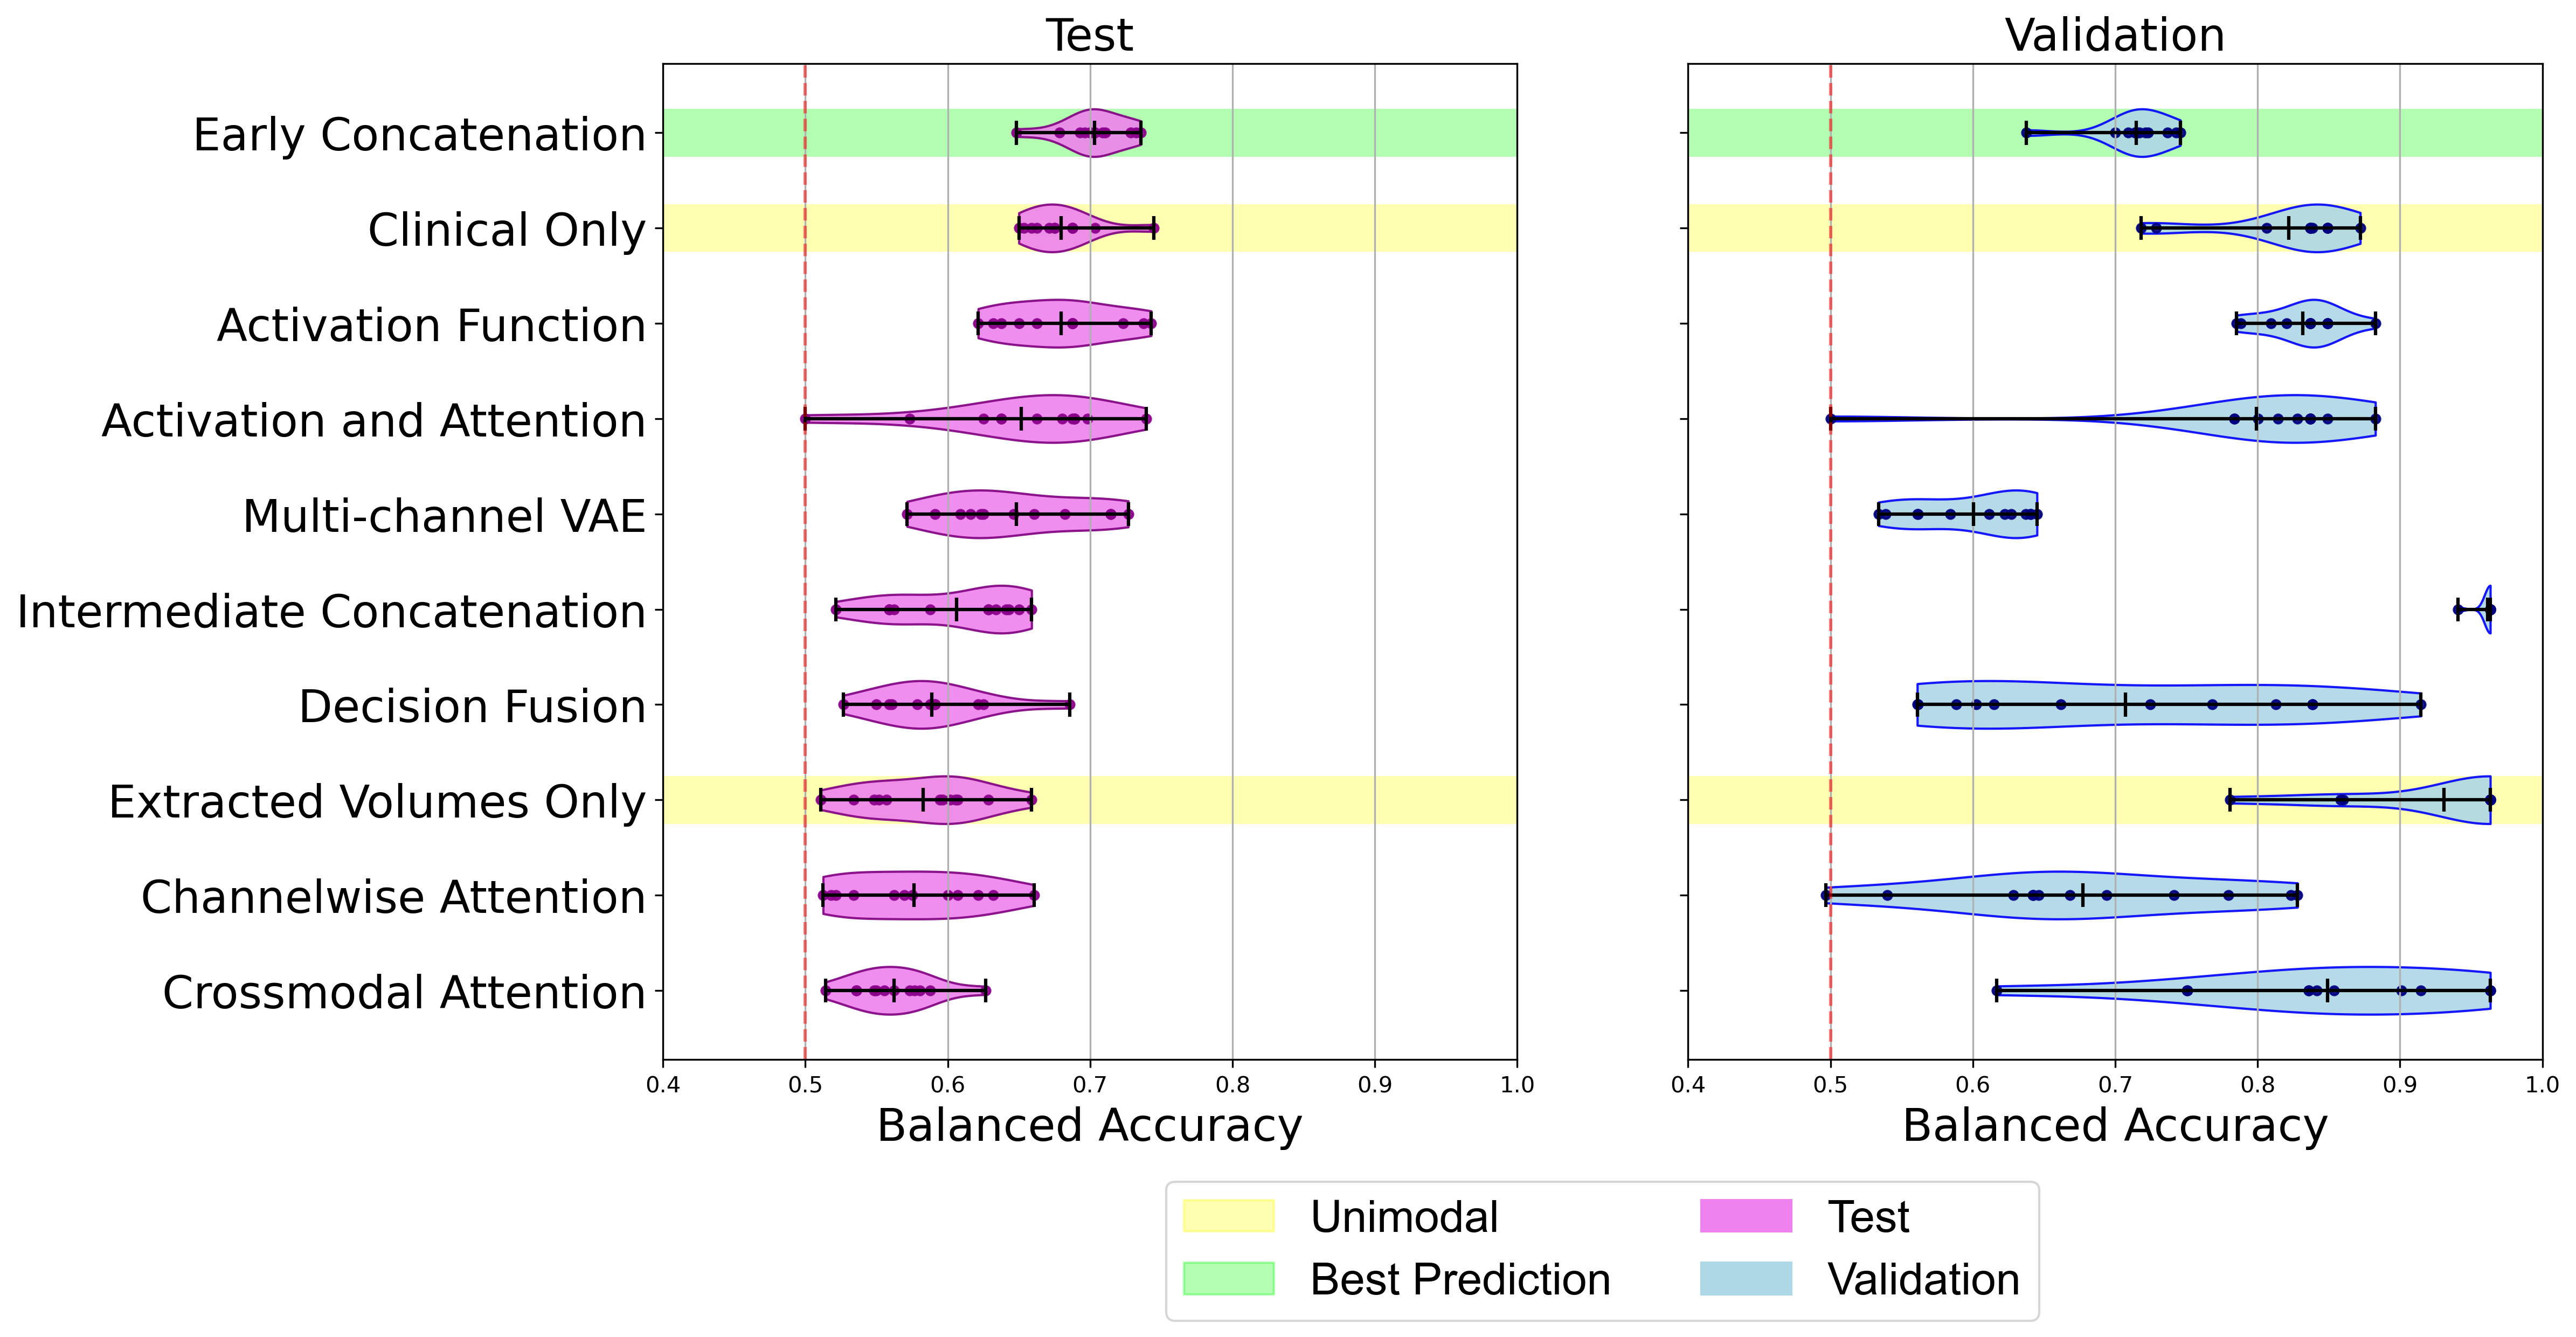
\includegraphics[width=1.2\linewidth]{figures/both_sites_together_balanced_accuracy_violin}
    \caption{Balanced accuracies of test set and validation set when sites trained together.}
    \label{fig:trainedtogetherviolin}
\end{figure}

\begin{table}[h]
\centering
\caption{Means and standard deviations of test metrics over repetitions of training on both sites. Bold is the best metric model.}
\label{tab:mnd_results}
\resizebox{\columnwidth}{!}{%
\begin{tabular}{lrrrrr}

 & \multicolumn{5}{c}{\textbf{Performance metric: mean (standard deviation)}} \\
\textbf{Method} & Balanced Accuracy & AUROC & Precision & Recall & F1 \\ \hline
 Early Concatenation & \textbf{0.703 (0.023)} & \textbf{0.815 (0.014)} & 0.846 (0.018) & 0.598 (0.065) & 0.698 (0.044) \\
Clinical Only & 0.680 (0.025) & 0.748 (0.052) & \textbf{0.870 (0.044)} & 0.493 (0.049) & 0.627 (0.040) \\
 Activation Function & 0.680 (0.039) & 0.744 (0.054) & 0.868 (0.048) & 0.493 (0.620) & 0.626 (0.057) \\
Activation and Attention & 0.652 (0.061) & 0.712 (0.093) & 0.772 (0.237) & 0.451 (0.158) & 0.566 (0.186) \\
Multi-channel VAE & 0.648 (0.049) & 0.727 (0.048) & 0.833 (0.075) & 0.474 (0.084) & 0.597 (0.073) \\
Intermediate Concatenation & 0.606 (0.044) & 0.663 (0.029) & 0.708 (0.030) & \textbf{0.764 (0.036)} & \textbf{0.735 (0.029)} \\
Decision Fusion & 0.589 (0.040) & 0.647 (0.042) & 0.737 (0.030) & 0.488 (0.166) & 0.567 (0.141) \\
Extracted Volumes Only & 0.583 (0.041) & 0.619 (0.038) & 0.695 (0.029) & 0.718 (0.101) & 0.703 (0.057) \\
Channelwise Attention & 0.576 (0.047) & 0.596 (0.052) & 0.730 (0.059) & 0.486 (0.193) & 0.558 (0.137) \\
Crossmodal Attention & 0.562 (0.028) & 0.610 (0.041) & 0.681 (0.025) & 0.720 (0.079) & 0.697 (0.032) \\

\end{tabular}
}
\end{table}


Results observations from the figure:
- Figure~\ref{fig:trainedtogetherviolin} has the models ranked by their balanced accuracy on the test set on the left, and the corresponding validation set balanced accuracy on the right, aggregated over the 5 validation folds. Distributions that make the violin plots are over the repetitions of training on both sites.
- Table~\ref{tab:mnd_results} shows the mean and standard deviations of the test metrics over the repetitions of training on both sites.
- Early concatenation performed the best with 70\% balanced accuracy and 81\% AUROC, with uni-modal clinical data and the activation functions models also performing well.
- The worst performing models had similar performed to each other at around 55\% accuracy: the attention models, imaging-only, and decision fusion.

Validation results
- Validation accuracies had a generally higher variance than the test accuracies, with the better test-performing models having validation accuracies with less spread.


Results observations from the table:
- Looking at the table, recall was above 50\% for only 4 out of the 10 models: imaging only, intermediate concatenation, early concatenation, and cross modal attention.
- Means that the methods weren't very good at accurately detecting long survivors


\subsection{Leave-site-out analysis}

\begin{figure}
    \centering
    \hspace*{-2cm}
    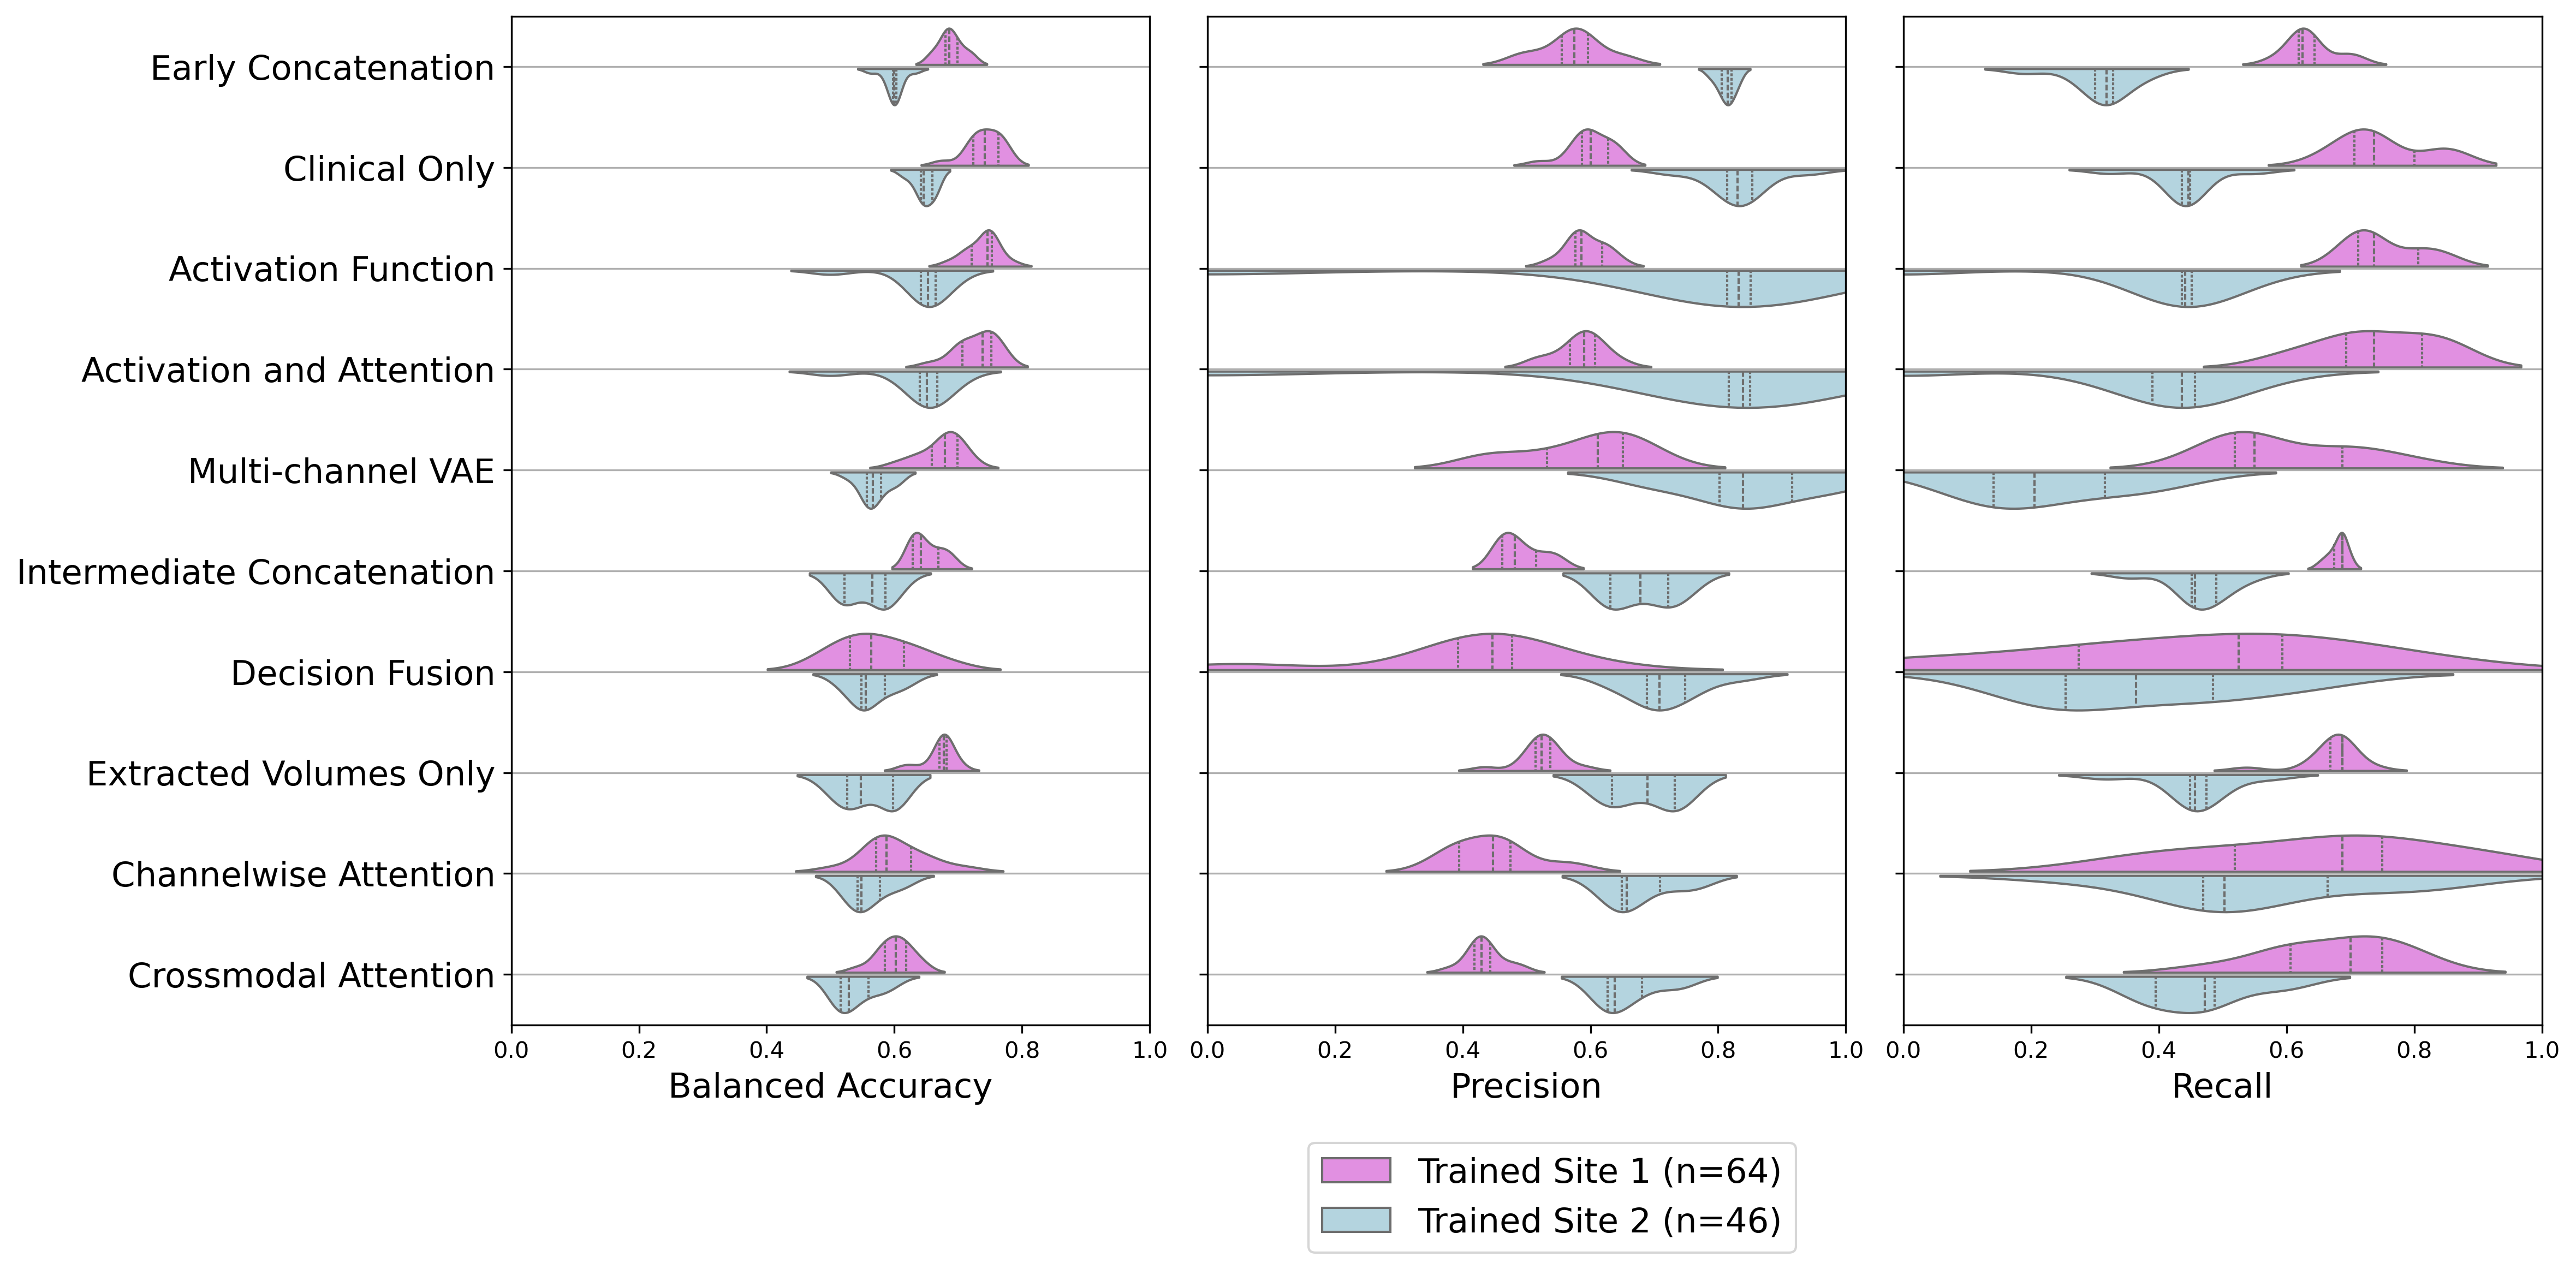
\includegraphics[width=1.2\textwidth]{figures/violinplot_site_effect}
    \caption{Effect of training on one site and testing on the other on the balanced accuracy, precision, and recall of the different models. Ordered by best to worst balanced accuracy of trained together.}
    \label{fig:site_effect}
\end{figure}

- Figure~\ref{fig:site_effect} shows the balanced accuracy of the different models when trained on one site and tested on the other.
- The models are ranked by their balanced accuracy when trained on both sites together.
- Training on site one generally resulted in better performance than training on site two, when looking at overall balanced accuracy.
- Training on ALS Biomarkers Study generally resulted in better precision, but worse recall
- Similar ranking on the methods too, but early concatenation doesn't perform as well as it does when trained on both sites together.


\section{Discussion}

\begin{figure}
    \centering
    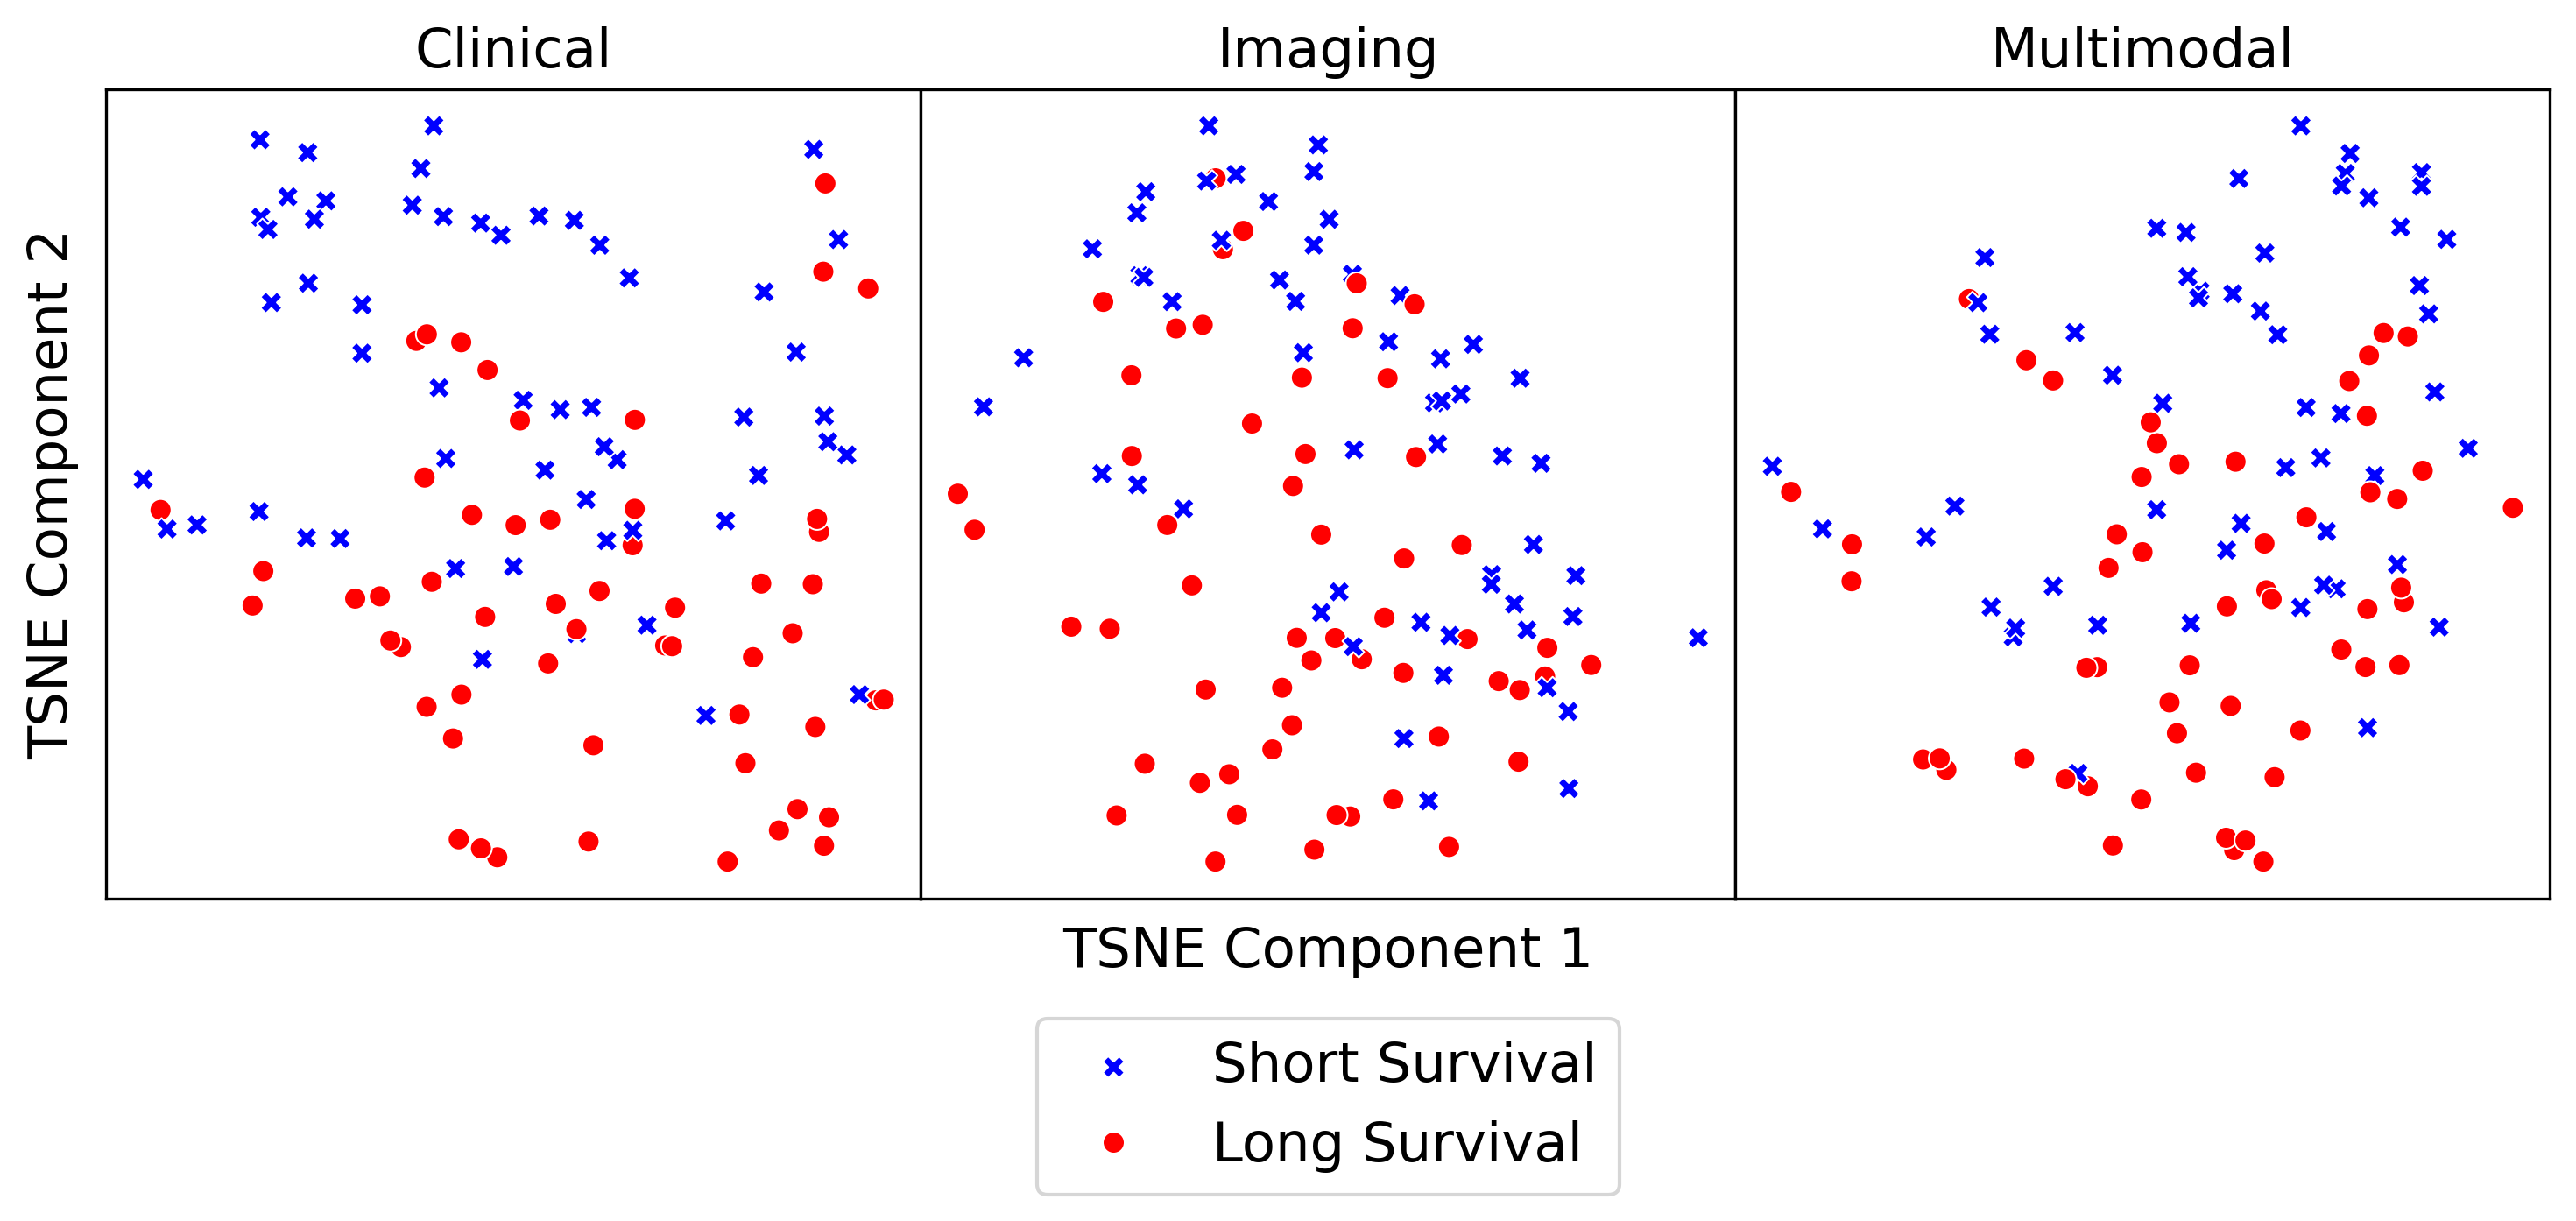
\includegraphics[width=0.9\textwidth]{figures/tsne_plot}
    \caption{TSNE with two components of the clinical, imaging, and multimodal data, split by survival category to illustrate the separability of the data.}
    \label{fig:tsne}
\end{figure}

Only one of the multimodal models was better than the clinical only model when comparing balanced accuracy: early concatenation, which is the most simple model.
Imaging only was one of the worst performing models, possibly because of the ratio of number of features to number of samples being high.
Figure~\ref{fig:trainedtogetherviolin} validation plot shows imaging overfitting on the validation set, with a much higher accuracy than the test set, probably because of the high number of features.

Generally, results aren't great: Figure~\ref{fig:tsne} shows the separability of the data from doing TSNE.
- Visually looks like clinical-only has the best separation but it's not obvious
- Can't expect to get excellent results
- This chapter is more of a proof of concept and early analysis, future work will look to improve the actual metrics


Overfitting on the validation set
- The distributions of validation fold balanced accuracies show that intermediate concatenation and imaging-only had very higher accuracy, but much lower test set accuracy, suggesting overfitting on the validation set.

Leave-site-out:
- Training on the higher sample size site (Milan) performs better than training on the lower sample size site (ALS Biomarkers Study)
- Early concatenation doesn't perform as well as it does when trained on both sites together, suggesting that it may be overfitting on the Milan data
- Statistically significant differences between the sites in Table~\ref{tab:clinical_demographics_site} showed that the Milan patients had different clinical features to the Essex patients, which may have meant the results were ungeneralisable to ALS Biomarkers Study.
- However, the overall results are similar to the trained together results, either suggesting that the models are generalisable to the ALS Biomarkers Study data or that model architecture is more important than the data used to train it.

Comparing models: how much does the model architecture affect the performance
- With more data in figure 5.1, the architecture does make a difference in the performance, ranging from around 55\% to 70\% balanced accuracy.
- Looking at how the number of parameters (a proxy for model complexity) is correlated with test model performance, there was no statistically significant correlation between the two for the metrics used in this analysis, using pearsons r.
- In figure 5.2, it looks like the data makes more of a difference in model performance than the model, especially when considering precision and recall.
- with a larger sample size, the model architecture may make more of a difference in the performance of the models, once the overfitting on the validation set is reduced.

\subsection{Limitations}
\begin{itemize}
    \item Limitations on sample size
    \item Evaluating on validation set rather than a completely external test set
    \item Predictive task of classification rather than regression: what if we used a regression task instead? Would that be more useful? It's a harder task so may require more data
    \item Limitation on using extracted brain volumes rather than raw MRI: what if the regions we've chosen aren't the most important ones? Subcortical regions have shown to have a role in MND, but we haven't included them here. *Look this up - the thalamus stuff*. However, whole image may introduce bias because further progressed patients may have worse quality scans.
    \item Two sites put together without harmonisation
    \item Using whole ALSFRS-R rather than individual components - not possible to get with Milan data
    \item Needs more hyperparameter tuning of the different models to see if they can be improved. Next steps would be to test different network architectures and hyperparameters to see if the results can be improved.
\end{itemize}

\section{Conclusion}
First look at multimodal data fusion in MND. What does it mean? What are the implications? What are the next steps?
\begin{itemize}
    \item If imaging + clinical is useful
    \begin{itemize}
        \item Let's add modalities
        \item Let's mix up the imaging preprocessing: DTI? Sub-cortical segmentation?
    \end{itemize}
    \item If imaging + clinical isn't useful
    \begin{itemize}
        \item Let's swap out the imaging for other modalities
        \item Let's try different machine learning models
        \item Let's mix up the imaging preprocessing: DTI? Sub-cortical segmentation?
    \end{itemize}
\end{itemize}
